\documentclass[a4paper,11pt]{article}
\usepackage[utf8]{inputenc}
\usepackage[T1]{fontenc}
\usepackage[margin=2.5cm]{geometry}
\usepackage{amsmath,amssymb,bm}
\usepackage{graphicx}
\usepackage[american]{circuitikz}
\usetikzlibrary{arrows.meta,positioning,calc,shapes.geometric}
\usepackage{booktabs}
\usepackage[hidelinks]{hyperref}
\setlength{\emergencystretch}{1.5em}

\newcommand{\La}{L_{\mathrm{arm}}}
\newcommand{\sgn}{\operatorname{sgn}}

\begin{document}

%======================================================================
\section{Mathematical Model For Furuta Pendulum}
%======================================================================

\begin{figure}[h]
  \centering
  \includegraphics[width=0.45\textwidth]{furuta_fig.png}
  \caption{Furuta Pendulum. The symbols in the figure correspond to the text as
  $I_0 \to J_0$, $L_0 \to \La$, $m_1 \to m$, $l_1 \to L_p$ and $\tau \to T_m$.}
  \label{fig:furuta}
\end{figure}

\subsection{1. Rotary Arm}
The kinetic energy of the rotary arm is
\begin{equation}
  T_0 = \frac{1}{2} J_0 \dot\theta_0^2 ,
\end{equation}
where $J_0$ is the moment of inertia of the arm and its hub about the motor axis. The inertia of the motor rotor and gearbox is added through the motor model in Section~\ref{sec:motor}.

Let the rotary arm be the reference. Therefore, its gravitational potential energy is taken as zero.
\begin{equation}
  U_0 = 0
\end{equation}

\subsection{2. Pendulum}
The pendulum is modeled using its mass $m$, located at a distance $L_p$ from the pivot, together with its moment of inertia $J_1$ about an axis through its centre of mass perpendicular to the pendulum. The arm length, from the motor axis to the pendulum pivot, is denoted by $\La$.

The angular coordinates are:
\begin{itemize}
  \item $\theta_0$: rotation angle of the horizontal arm about the vertical axis.
  \item $\theta_1$: pendulum angle measured from the upright vertical position.
\end{itemize}

The centre-of-mass position of the pendulum in the inertial frame is
\begin{equation}
\begin{aligned}
  x_x &= \La \cos\theta_0 - L_p \sin\theta_1 \sin\theta_0 ,\\
  x_y &= \La \sin\theta_0 + L_p \sin\theta_1 \cos\theta_0 ,\\
  x_z &= L_p \cos\theta_1 .
\end{aligned}
\label{eq:pos}
\end{equation}

\subsubsection{Velocity of the Pendulum Center of Mass}
Differentiating the position coordinates with respect to time gives
\begin{equation}
\begin{aligned}
  \dot x_x = {}& -\La \sin\theta_0\,\dot\theta_0\\
  & - L_p \cos\theta_1 \sin\theta_0\,\dot\theta_1\\
  & - L_p \sin\theta_1 \cos\theta_0\,\dot\theta_0 ,
\end{aligned}
\end{equation}
\begin{equation}
\begin{aligned}
  \dot x_y = {}& \La \cos\theta_0\,\dot\theta_0\\
  & + L_p \cos\theta_1 \cos\theta_0\,\dot\theta_1\\
  & - L_p \sin\theta_1 \sin\theta_0\,\dot\theta_0 ,
\end{aligned}
\end{equation}
\begin{equation}
  \dot x_z = -L_p \sin\theta_1\,\dot\theta_1 .
\end{equation}
The squared magnitude of the velocity is
\begin{equation}
  v^2 = \dot x_x^2 + \dot x_y^2 + \dot x_z^2 .
\end{equation}
Solving that equation using MATLAB
\begin{equation}
\begin{aligned}
  v^2 = {}& \La^2 \dot\theta_0^2 + L_p^2 \dot\theta_1^2\\
  & + L_p^2 \dot\theta_0^2 \sin^2\theta_1\\
  & + 2 \La L_p \dot\theta_0 \dot\theta_1 \cos\theta_1 .
\end{aligned}
\label{eq:v2}
\end{equation}
This expression includes the three-dimensional motion of the pendulum centre of mass.

\subsubsection{Kinetic Energy of the Pendulum}
The angular velocity of the pendulum is the sum of the arm rotation $\dot\theta_0$ about the vertical axis and the pendulum rotation $\dot\theta_1$ about the arm axis. Resolving it along the principal axes of the pendulum gives:
\begin{itemize}
  \item $\dot\theta_1$ about the arm axis, which is perpendicular to the pendulum;
  \item $\dot\theta_0 \sin\theta_1$ about the axis perpendicular to both the arm and the pendulum;
  \item $\dot\theta_0 \cos\theta_1$ about the long axis of the pendulum.
\end{itemize}
The pendulum is treated as a slender rod, so its moment of inertia about its long axis is neglected and $J_1$ applies to both perpendicular axes. The rotational kinetic energy of the pendulum is therefore
\begin{equation}
  T_{\mathrm{rotational}} = \frac{1}{2} J_1 \left(\dot\theta_1^2 + \dot\theta_0^2 \sin^2\theta_1\right).
  \label{eq:Trot}
\end{equation}
The translational kinetic energy is
\begin{equation}
  T_{\mathrm{translational}} = \frac{1}{2} m v^2 .
\end{equation}
Substituting Eq.~\eqref{eq:v2} gives
\begin{equation}
  T_{\mathrm{translational}} = \frac{1}{2} m \left[\left(\dot\theta_0 \La\right)^2 + \left(\dot\theta_1 L_p\right)^2 + \left(\dot\theta_0 L_p \sin\theta_1\right)^2 + 2 L_p \La \dot\theta_0 \dot\theta_1 \cos\theta_1\right]
\end{equation}
therefore, after expanding the terms
\begin{equation}
\begin{aligned}
  T_{\mathrm{translational}} = {}& \frac{1}{2} m \La^2 \dot\theta_0^2 + \frac{1}{2} m L_p^2 \dot\theta_1^2\\
  & + \frac{1}{2} m L_p^2 \dot\theta_0^2 \sin^2\theta_1\\
  & + m \La L_p \dot\theta_0 \dot\theta_1 \cos\theta_1 .
\end{aligned}
\end{equation}
Therefore, the total kinetic energy of the pendulum is
\begin{equation}
\begin{aligned}
  T_1 = {}& \frac{1}{2} m \La^2 \dot\theta_0^2 + \frac{1}{2}\left(J_1 + m L_p^2\right)\dot\theta_1^2\\
  & + \frac{1}{2}\left(J_1 + m L_p^2\right)\dot\theta_0^2 \sin^2\theta_1\\
  & + m \La L_p \dot\theta_0 \dot\theta_1 \cos\theta_1 .
\end{aligned}
\label{eq:T1}
\end{equation}

\subsubsection{Potential Energy of the Pendulum}
Taking the zero of gravitational potential energy at the horizontal plane through the pivot, the vertical coordinate is $x_z = L_p \cos\theta_1$. Hence,
\begin{equation}
  U_1 = m g L_p \cos\theta_1 .
\end{equation}

\subsection{3. Total Kinetic Energy and Lagrangian}
The total kinetic energy of the system is obtained by adding the arm kinetic energy and the pendulum kinetic energy:
\begin{equation}
  T = T_0 + T_1 .
\end{equation}
Substituting $T_0$ and Eq.~\eqref{eq:T1} gives
\begin{equation}
\begin{aligned}
  T = {}& \frac{1}{2}\left(J_0 + m \La^2\right)\dot\theta_0^2\\
  & + \frac{1}{2}\left(J_1 + m L_p^2\right)\dot\theta_1^2\\
  & + \frac{1}{2}\left(J_1 + m L_p^2\right)\dot\theta_0^2 \sin^2\theta_1\\
  & + m \La L_p \dot\theta_0 \dot\theta_1 \cos\theta_1 .
\end{aligned}
\label{eq:T}
\end{equation}
The total potential energy is
\begin{equation}
  U = U_0 + U_1 .
\end{equation}
Therefore,
\begin{equation}
  U = m g L_p \cos\theta_1 .
  \label{eq:U}
\end{equation}
The Lagrangian is defined as
\begin{equation}
  \mathcal{L} = T - U .
\end{equation}
Substituting Eqs.~\eqref{eq:T} and~\eqref{eq:U}, the complete Lagrangian becomes
\begin{equation}
\begin{aligned}
  \mathcal{L} = {}& \frac{1}{2}\left(J_0 + m \La^2\right)\dot\theta_0^2\\
  & + \frac{1}{2}\left(J_1 + m L_p^2\right)\dot\theta_1^2\\
  & + \frac{1}{2}\left(J_1 + m L_p^2\right)\dot\theta_0^2 \sin^2\theta_1\\
  & + m \La L_p \dot\theta_0 \dot\theta_1 \cos\theta_1\\
  & - m g L_p \cos\theta_1 .
\end{aligned}
\label{eq:Lag}
\end{equation}

\subsection{4. Euler--Lagrange Equations}
The Euler--Lagrange equation for each generalized coordinate is
\begin{equation}
  \frac{d}{dt}\left(\frac{\partial \mathcal{L}}{\partial \dot q_i}\right) - \frac{\partial \mathcal{L}}{\partial q_i} = Q_i
\end{equation}
where the generalized coordinates are $\theta_0$ and $\theta_1$. Here, $T_m$ is the motor torque applied to the arm, while $b_0$ and $b_1$ are the viscous damping coefficients at the arm and pendulum joints, respectively.

\subsubsection{Equation of Motion for \texorpdfstring{$\theta_0$}{theta0}}
First, differentiate the Lagrangian with respect to $\dot\theta_0$:
\begin{equation}
\begin{aligned}
  \frac{\partial \mathcal{L}}{\partial \dot\theta_0} = {}& \left(J_0 + m \La^2\right)\dot\theta_0\\
  & + \left(J_1 + m L_p^2\right)\dot\theta_0 \sin^2\theta_1\\
  & + m \La L_p \dot\theta_1 \cos\theta_1 .
\end{aligned}
\end{equation}
Differentiating with respect to time gives
\begin{equation}
\begin{aligned}
  \frac{d}{dt}\left(\frac{\partial \mathcal{L}}{\partial \dot\theta_0}\right) = {}& \left(J_0 + m \La^2\right)\ddot\theta_0\\
  & + \left(J_1 + m L_p^2\right)\sin^2\theta_1\,\ddot\theta_0\\
  & + 2\left(J_1 + m L_p^2\right)\sin\theta_1 \cos\theta_1\,\dot\theta_0 \dot\theta_1\\
  & + m \La L_p \cos\theta_1\,\ddot\theta_1\\
  & - m \La L_p \sin\theta_1\,\dot\theta_1^2 .
\end{aligned}
\end{equation}
Because the Lagrangian does not explicitly depend on $\theta_0$,
\begin{equation}
  \frac{\partial \mathcal{L}}{\partial \theta_0} = 0 .
\end{equation}
The generalized torque is
\begin{equation}
  Q_0 = T_m - b_0 \dot\theta_0
\end{equation}
Substituting into the Euler--Lagrange equation gives the arm equation of motion
\begin{equation}
\begin{aligned}
  & \left(J_0 + m \La^2 + \left(J_1 + m L_p^2\right)\sin^2\theta_1\right)\ddot\theta_0\\
  & + m \La L_p \cos\theta_1\,\ddot\theta_1\\
  & + 2\left(J_1 + m L_p^2\right)\sin\theta_1 \cos\theta_1\,\dot\theta_0 \dot\theta_1\\
  & - m \La L_p \sin\theta_1\,\dot\theta_1^2 = T_m - b_0 \dot\theta_0 .
\end{aligned}
\end{equation}
Rearranging, the nonlinear arm equation becomes
\begin{equation}
\begin{aligned}
  & \left(J_0 + m \La^2 + \left(J_1 + m L_p^2\right)\sin^2\theta_1\right)\ddot\theta_0\\
  & + m \La L_p \cos\theta_1\,\ddot\theta_1\\
  & + 2\left(J_1 + m L_p^2\right)\sin\theta_1 \cos\theta_1\,\dot\theta_0 \dot\theta_1\\
  & - m \La L_p \sin\theta_1\,\dot\theta_1^2 + b_0 \dot\theta_0 = T_m .
\end{aligned}
\label{eq:arm_nl}
\end{equation}

\subsubsection{Equation of Motion for \texorpdfstring{$\theta_1$}{theta1}}
Differentiate the Lagrangian with respect to $\dot\theta_1$:
\begin{equation}
  \frac{\partial \mathcal{L}}{\partial \dot\theta_1} = \left(J_1 + m L_p^2\right)\dot\theta_1 + m \La L_p \cos\theta_1\,\dot\theta_0 .
\end{equation}
Differentiating with respect to time
\begin{equation}
\begin{aligned}
  \frac{d}{dt}\left(\frac{\partial \mathcal{L}}{\partial \dot\theta_1}\right) = {}& \left(J_1 + m L_p^2\right)\ddot\theta_1\\
  & + m \La L_p \cos\theta_1\,\ddot\theta_0\\
  & - m \La L_p \sin\theta_1\,\dot\theta_0 \dot\theta_1 .
\end{aligned}
\end{equation}
Next, differentiate the Lagrangian with respect to $\theta_1$:
\begin{equation}
\begin{aligned}
  \frac{\partial \mathcal{L}}{\partial \theta_1} = {}& \left(J_1 + m L_p^2\right)\dot\theta_0^2 \sin\theta_1 \cos\theta_1\\
  & - m \La L_p \dot\theta_0 \dot\theta_1 \sin\theta_1\\
  & + m g L_p \sin\theta_1 .
\end{aligned}
\end{equation}
The generalized torque for the pendulum is
\begin{equation}
  Q_1 = -b_1 \dot\theta_1
\end{equation}
Applying the Euler--Lagrange equation for $\theta_1$, the terms $m \La L_p \sin\theta_1\,\dot\theta_0 \dot\theta_1$ cancel and
\begin{equation}
\begin{aligned}
  & \left(J_1 + m L_p^2\right)\ddot\theta_1\\
  & + m \La L_p \cos\theta_1\,\ddot\theta_0\\
  & - \left(J_1 + m L_p^2\right)\sin\theta_1 \cos\theta_1\,\dot\theta_0^2\\
  & - m g L_p \sin\theta_1 = -b_1 \dot\theta_1 .
\end{aligned}
\end{equation}
Rearranging, the nonlinear pendulum equation becomes
\begin{equation}
\begin{aligned}
  & \left(J_1 + m L_p^2\right)\ddot\theta_1\\
  & + m \La L_p \cos\theta_1\,\ddot\theta_0\\
  & - \left(J_1 + m L_p^2\right)\sin\theta_1 \cos\theta_1\,\dot\theta_0^2\\
  & + b_1 \dot\theta_1 - m g L_p \sin\theta_1 = 0 .
\end{aligned}
\label{eq:pend_nl}
\end{equation}

\subsection{5. Linearization Around the Upright Equilibrium}
The upright equilibrium corresponds to
\begin{equation}
  \theta_1 = 0, \qquad \dot\theta_0 = \dot\theta_1 = 0, \qquad \ddot\theta_0 = \ddot\theta_1 = 0 .
\end{equation}
For small deviations about this equilibrium, use the approximations
\begin{equation}
  \sin\theta_1 \approx \theta_1, \qquad \cos\theta_1 \approx 1, \qquad \sin^2\theta_1 \approx 0 .
\end{equation}
Terms containing products of small deviations, velocities, or accelerations are neglected.

\subsubsection{Linearization of the Arm Equation}
Starting from Eq.~\eqref{eq:arm_nl}, the terms containing $\sin^2\theta_1$ and products of small quantities are neglected. With $\cos\theta_1 \approx 1$, the linearized arm equation is
\begin{equation}
  \left(J_0 + m \La^2\right)\ddot\theta_0 + m \La L_p \ddot\theta_1 + b_0 \dot\theta_0 = T_m .
\end{equation}

\subsubsection{Linearization of the Pendulum Equation}
Starting from Eq.~\eqref{eq:pend_nl}, the term containing $\dot\theta_0^2$ is neglected, and $\sin\theta_1 \approx \theta_1$ and $\cos\theta_1 \approx 1$ are applied. Thus,
\begin{equation}
  m \La L_p \ddot\theta_0 + \left(J_1 + m L_p^2\right)\ddot\theta_1 + b_1 \dot\theta_1 - m g L_p \theta_1 = 0 .
\end{equation}
The linearized equations are therefore
\begin{equation}
\begin{aligned}
  \left(J_0 + m \La^2\right)\ddot\theta_0 + m \La L_p \ddot\theta_1 + b_0 \dot\theta_0 &= T_m ,\\
  m \La L_p \ddot\theta_0 + \left(J_1 + m L_p^2\right)\ddot\theta_1 + b_1 \dot\theta_1 - m g L_p \theta_1 &= 0 .
\end{aligned}
\label{eq:lin}
\end{equation}

\subsection{6. Deriving the Angular Accelerations}
From the first equation of~\eqref{eq:lin},
\begin{equation}
  \ddot\theta_0 = \frac{T_m - b_0 \dot\theta_0 - m \La L_p \ddot\theta_1}{J_0 + m \La^2}
  \label{eq:acc0_impl}
\end{equation}
and from the second equation of~\eqref{eq:lin},
\begin{equation}
  \ddot\theta_1 = \frac{m g L_p \theta_1 - b_1 \dot\theta_1 - m \La L_p \ddot\theta_0}{J_1 + m L_p^2}
  \label{eq:acc1_impl}
\end{equation}
Substituting Eq.~\eqref{eq:acc1_impl} into Eq.~\eqref{eq:acc0_impl} and multiplying by $\left(J_0 + m \La^2\right)\left(J_1 + m L_p^2\right)$ gives
\begin{equation}
\begin{aligned}
  & \left[\left(J_0 + m \La^2\right)\left(J_1 + m L_p^2\right) - m^2 \La^2 L_p^2\right]\ddot\theta_0\\
  & \qquad = \left(J_1 + m L_p^2\right)\left(T_m - b_0 \dot\theta_0\right) - m \La L_p \left(m g L_p \theta_1 - b_1 \dot\theta_1\right).
\end{aligned}
\end{equation}
Similarly, substituting Eq.~\eqref{eq:acc0_impl} into Eq.~\eqref{eq:acc1_impl} gives
\begin{equation}
\begin{aligned}
  & \left[\left(J_0 + m \La^2\right)\left(J_1 + m L_p^2\right) - m^2 \La^2 L_p^2\right]\ddot\theta_1\\
  & \qquad = -m \La L_p \left(T_m - b_0 \dot\theta_0\right) + \left(J_0 + m \La^2\right)\left(m g L_p \theta_1 - b_1 \dot\theta_1\right).
\end{aligned}
\end{equation}
Define
\begin{equation}
  \Delta = \left(J_0 + m \La^2\right)\left(J_1 + m L_p^2\right) - m^2 \La^2 L_p^2 = J_0 J_1 + J_0 m L_p^2 + J_1 m \La^2
  \label{eq:Delta}
\end{equation}
which is always positive, and let
\begin{equation}
  a = \frac{1}{\Delta}
\end{equation}
The angular accelerations are then
\begin{equation}
\begin{aligned}
  \ddot\theta_0 = {}& a\left(J_1 + m L_p^2\right)\left(T_m - b_0 \dot\theta_0\right)\\
  & - a\, m \La L_p \left(m g L_p \theta_1 - b_1 \dot\theta_1\right)
\end{aligned}
\label{eq:acc0}
\end{equation}
\begin{equation}
\begin{aligned}
  \ddot\theta_1 = {}& -a\, m \La L_p \left(T_m - b_0 \dot\theta_0\right)\\
  & + a\left(J_0 + m \La^2\right)\left(m g L_p \theta_1 - b_1 \dot\theta_1\right)
\end{aligned}
\label{eq:acc1}
\end{equation}

\subsection{7. State-Space Representation}
The four state variables are
\begin{equation}
  \mathbf{x} = \begin{bmatrix} \theta_0 \\ \theta_1 \\ \dot\theta_0 \\ \dot\theta_1 \end{bmatrix}
\end{equation}
The state derivative vector is
\begin{equation}
  \dot{\mathbf{x}} = \begin{bmatrix} \dot\theta_0 \\ \dot\theta_1 \\ \ddot\theta_0 \\ \ddot\theta_1 \end{bmatrix}
\end{equation}
The input is the motor torque,
\begin{equation}
  u = T_m
\end{equation}
The linear state-space model is
\begin{equation}
  \dot{\mathbf{x}} = A\mathbf{x} + Bu
\end{equation}

\subsubsection{System Matrix \texorpdfstring{$A$}{A}}
Reading the coefficients of Eqs.~\eqref{eq:acc0} and~\eqref{eq:acc1}, the state matrix is
\begin{equation}
\boxed{
A = \begin{bmatrix}
0 & 0 & 1 & 0\\
0 & 0 & 0 & 1\\
0 & -a\, m^2 g \La L_p^2 & -a\, b_0 \left(J_1 + m L_p^2\right) & a\, m \La L_p b_1\\
0 & a\, m g L_p \left(J_0 + m \La^2\right) & a\, m \La L_p b_0 & -a\left(J_0 + m \La^2\right) b_1
\end{bmatrix}.
}
\end{equation}

\subsubsection{Input Matrix \texorpdfstring{$B$}{B}}
Since the input is the motor torque $u = T_m$, the input matrix is
\begin{equation}
\boxed{
B = \begin{bmatrix} 0 \\ 0 \\ a\left(J_1 + m L_p^2\right) \\ -a\, m \La L_p \end{bmatrix}.
}
\end{equation}
Therefore, the complete state-space model is
\begin{equation}
\boxed{\dot{\mathbf{x}} = A\mathbf{x} + Bu .}
\end{equation}
\begin{equation}
\begin{aligned}
\begin{bmatrix} \dot\theta_0 \\ \dot\theta_1 \\ \ddot\theta_0 \\ \ddot\theta_1 \end{bmatrix}
= {}&
\begin{bmatrix}
0 & 0 & 1 & 0\\
0 & 0 & 0 & 1\\
0 & -a\, m^2 g L_p^2 \La & -a\left(J_1 + m L_p^2\right) b_0 & a\, m \La L_p b_1\\
0 & a\, m g L_p \left(J_0 + m \La^2\right) & a\, m \La L_p b_0 & -a\left(J_0 + m \La^2\right) b_1
\end{bmatrix}
\begin{bmatrix} \theta_0 \\ \theta_1 \\ \dot\theta_0 \\ \dot\theta_1 \end{bmatrix}\\
& + \begin{bmatrix} 0 \\ 0 \\ a\left(J_1 + m L_p^2\right) \\ -a\, m \La L_p \end{bmatrix} T_m
\end{aligned}
\label{eq:ss4T}
\end{equation}

\subsection{8. Output Equations}
Both joint angles are measured as outputs: $\theta_0$ by the motor encoder (11 PPR quadrature encoder on the motor shaft, read in $\times4$ mode) and $\theta_1$ by the pendulum encoder (AS5600 12-bit magnetic angle sensor). Therefore, define
\begin{equation}
  \mathbf{y} = \begin{bmatrix} \theta_0 \\ \theta_1 \end{bmatrix}.
\end{equation}
The output equation is
\begin{equation}
  \mathbf{y} = C\mathbf{x} + Du ,
\end{equation}
where
\begin{equation}
  C = \begin{bmatrix} 1 & 0 & 0 & 0 \\ 0 & 1 & 0 & 0 \end{bmatrix}, \qquad
  D = \begin{bmatrix} 0 \\ 0 \end{bmatrix}.
\end{equation}

\paragraph{Sign convention.} Eq.~\eqref{eq:pos} fixes the positive directions: $\theta_0 > 0$ is counter-clockwise when viewed from above, and $\theta_1 > 0$ means the pendulum leans in the direction the arm tip moves when $\theta_0$ increases. Consequently $B_4 < 0$: a positive motor torque initially tips the pendulum backward. The counting direction of the motor encoder, the sign of the pendulum encoder and the motor polarity must follow this convention.

%======================================================================
\section{DC Motor Model}
\label{sec:motor}
%======================================================================
The arm is driven by a brushed DC gearmotor. The motor driver (TB6612FNG dual H-bridge) applies a PWM voltage to the armature, commanded by the microcontroller (ESP32-S3). This section derives the torque $T_m$ delivered to the arm as a function of the armature voltage $V$, including the armature inductance. The model is shown in Fig.~\ref{fig:motor}.

\begin{figure}[h]
\centering
\begin{circuitikz}[scale=0.9, transform shape]
  % electrical side
  \draw (0,0) to[V, l=$V$, invert] (0,3)
        to[R, l=$R_m$, i>^=$i$] (3,3)
        to[L, l=$L_m$] (5.5,3)
        to[V, l_={$e_b = K_e\,\omega_m$}] (5.5,0)
        -- (0,0);
  \node[align=center, font=\small] at (2.75,-0.8) {Armature circuit};
  % mechanical side
  \draw[thick, fill=gray!15] (7.6,0.7) rectangle (9.4,2.3);
  \node[align=center, font=\small] at (8.5,1.5) {Rotor\\$J_m,\ b_m$};
  \draw[dashed, -{Stealth}] (6.0,1.5) -- (7.6,1.5);
  \node[font=\scriptsize, above] at (6.8,1.55) {$T_e = K_t\, i$};
  \draw[very thick] (9.4,1.5) -- (10.2,1.5);
  \node[font=\scriptsize, above] at (9.8,1.55) {$\omega_m$};
  \node[font=\scriptsize, below] at (9.8,1.45) {$T_g$};
  \draw[thick, fill=gray!15] (10.2,0.5) rectangle (11.9,2.5);
  \node[align=center, font=\small] at (11.05,1.5) {Gearbox\\$N\!:\!1,\ \eta_g$};
  \draw[very thick] (11.9,1.5) -- (12.9,1.5);
  \node[font=\scriptsize, above] at (12.4,1.55) {$\dot\theta_0$};
  \node[font=\scriptsize, below] at (12.4,1.45) {$T_m$};
  \draw[thick, fill=gray!35] (12.9,1.2) rectangle (14.1,1.8);
  \node[font=\small, below] at (13.5,1.15) {Arm};
  \draw[-{Stealth}, thick] (13.5,2.0) arc[start angle=200, end angle=-20, radius=0.35];
  \node[font=\scriptsize, above] at (13.5,2.45) {$\theta_0$};
  \node[align=center, font=\small] at (10.85,-0.8) {Rotor, gearbox and arm};
\end{circuitikz}
\caption{DC gearmotor model. The motor driver supplies the armature voltage $V$; the back-EMF $e_b$ and the electromagnetic torque $T_e$ couple the armature circuit to the rotor, which drives the arm through the gearbox.}
\label{fig:motor}
\end{figure}

\subsection{1. Armature Circuit}
The armature is modeled as a resistance $R_m$ in series with an inductance $L_m$ and the back-EMF $e_b$. Applying Kirchhoff's voltage law around the loop of Fig.~\ref{fig:motor},
\begin{equation}
  V - R_m i - L_m \frac{di}{dt} - e_b = 0 ,
\end{equation}
therefore,
\begin{equation}
  V = R_m i + L_m \frac{di}{dt} + e_b ,
  \label{eq:kvl}
\end{equation}
where $i$ is the armature current. The back-EMF is proportional to the rotor speed $\omega_m$:
\begin{equation}
  e_b = K_e\, \omega_m .
  \label{eq:emf}
\end{equation}

\subsection{2. Electromagnetic Torque}
The torque produced on the rotor is proportional to the armature current:
\begin{equation}
  T_e = K_t\, i .
\end{equation}
The electrical power absorbed by the back-EMF equals the mechanical power developed by the rotor:
\begin{equation}
  e_b\, i = T_e\, \omega_m \;\Rightarrow\; K_e\, \omega_m\, i = K_t\, i\, \omega_m \;\Rightarrow\; K_t = K_e ,
  \label{eq:KtKe}
\end{equation}
with $K_t$ in N\,m/A and $K_e$ in V\,s/rad.

\subsection{3. Rotor Dynamics}
Let $J_m$ be the rotor inertia, $b_m$ the rotor viscous friction coefficient, and $T_g$ the torque the rotor delivers to the gearbox input. Newton's second law for the rotor gives
\begin{equation}
  J_m \dot\omega_m = K_t\, i - b_m \omega_m - T_g ,
\end{equation}
therefore,
\begin{equation}
  T_g = K_t\, i - J_m \dot\omega_m - b_m \omega_m .
  \label{eq:rotor}
\end{equation}

\subsection{4. Gearbox}
With gear ratio $N$ (motor revolutions per output revolution), the rotor and output speeds are related by
\begin{equation}
  \omega_m = N \dot\theta_0, \qquad \dot\omega_m = N \ddot\theta_0 .
  \label{eq:gear}
\end{equation}
The gearbox losses are modeled by an efficiency $\eta_g$ ($0 < \eta_g \le 1$), so the output power is $\eta_g$ times the input power:
\begin{equation}
  T_{\mathrm{out}}\, \dot\theta_0 = \eta_g\, T_g\, \omega_m \;\Rightarrow\; T_{\mathrm{out}} = \eta_g N\, T_g .
\end{equation}
The dry friction of the brushes and the gear mesh is represented by a Coulomb torque $\tau_c$ acting at the output shaft, so the torque applied to the arm is
\begin{equation}
  T_m = \eta_g N\, T_g - \tau_c \sgn(\dot\theta_0) .
  \label{eq:Tout}
\end{equation}

\subsection{5. Motor Torque Acting on the Arm}
Substituting Eqs.~\eqref{eq:rotor} and~\eqref{eq:gear} into Eq.~\eqref{eq:Tout} gives
\begin{equation}
  T_m = \eta_g N K_t\, i - \eta_g N^2 J_m\, \ddot\theta_0 - \eta_g N^2 b_m\, \dot\theta_0 - \tau_c \sgn(\dot\theta_0) .
\end{equation}
Similarly, substituting Eqs.~\eqref{eq:emf} and~\eqref{eq:gear} into Eq.~\eqref{eq:kvl} gives the armature equation in terms of the output speed. Define the output-referred motor parameters
\begin{equation}
  K_\tau = \eta_g N K_t, \qquad K_b = N K_e, \qquad J_{mo} = \eta_g N^2 J_m, \qquad b_{mo} = \eta_g N^2 b_m .
  \label{eq:outref}
\end{equation}
The motor model is then
\begin{equation}
\boxed{
\begin{aligned}
  T_m &= K_\tau\, i - J_{mo}\, \ddot\theta_0 - b_{mo}\, \dot\theta_0 - \tau_c \sgn(\dot\theta_0)\\
  L_m \frac{di}{dt} &= V - R_m i - K_b\, \dot\theta_0
\end{aligned}
}
\label{eq:motor}
\end{equation}
From Eq.~\eqref{eq:KtKe}, $K_\tau = \eta_g K_b$, so the identified values must satisfy $0 < K_\tau / K_b \le 1$.

\subsection{6. Motor Driver Voltage}
With PWM duty cycle $d \in [-1, 1]$ and supply voltage $V_s$, the average armature voltage applied by the motor driver (TB6612FNG) is
\begin{equation}
  V = d\, V_s .
  \label{eq:duty}
\end{equation}
This holds when the PWM period is much shorter than the electrical time constant $\tau_e$ of Eq.~\eqref{eq:taus}, so the current responds to the average voltage. The on-resistance of the H-bridge is in series with the armature and is lumped into $R_m$.

\subsection{7. Motor Transfer Functions}
For the motor alone, driving only the hub of inertia $J_L$ on the output shaft, $T_m = J_L \ddot\theta_0$. With the Coulomb friction neglected, $\omega = \dot\theta_0$, $J = J_{mo} + J_L$ and $b = b_{mo}$, Eq.~\eqref{eq:motor} becomes
\begin{equation}
  J \dot\omega + b\, \omega = K_\tau\, i, \qquad L_m \frac{di}{dt} + R_m i = V - K_b\, \omega .
\end{equation}
Taking the Laplace transform with zero initial conditions,
\begin{equation}
  \Omega(s) = \frac{K_\tau}{J s + b}\, I(s), \qquad I(s) = \frac{V(s) - K_b\, \Omega(s)}{L_m s + R_m} .
\end{equation}
Eliminating $I(s)$ gives
\begin{equation}
\boxed{
  \frac{\Omega(s)}{V(s)} = \frac{K_\tau}{(L_m s + R_m)(J s + b) + K_\tau K_b}, \qquad
  \frac{I(s)}{V(s)} = \frac{J s + b}{(L_m s + R_m)(J s + b) + K_\tau K_b}
}
\label{eq:motorTF}
\end{equation}
The characteristic polynomial is
\begin{equation}
  L_m J s^2 + \left(L_m b + R_m J\right)s + \left(R_m b + K_\tau K_b\right) ,
\end{equation}
and the electrical and mechanical time constants are
\begin{equation}
  \tau_e = \frac{L_m}{R_m}, \qquad \tau_m = \frac{R_m J}{R_m b + K_\tau K_b} .
  \label{eq:taus}
\end{equation}

%======================================================================
\section{Full Electromechanical Model}
\label{sec:full}
%======================================================================

\subsection{1. Substituting the Motor Model into the Pendulum Model}
Substituting $T_m$ from Eq.~\eqref{eq:motor} into the arm equation~\eqref{eq:arm_nl}, the terms $J_{mo}\ddot\theta_0$, $b_{mo}\dot\theta_0$ and $\tau_c \sgn(\dot\theta_0)$ move to the left-hand side. To keep the equations compact, define
\begin{equation}
  J_a = J_0 + J_{mo} + m \La^2, \qquad J_p = J_1 + m L_p^2, \qquad h = m \La L_p, \qquad B_{eq} = b_0 + b_{mo} ,
  \label{eq:short}
\end{equation}
where $J_a$ is the total inertia about the motor axis (arm, reflected rotor and pendulum mass at the arm tip), $J_p$ is the pendulum inertia about its pivot, $h$ is the inertial coupling, and $B_{eq}$ is the total viscous friction at the arm. The full nonlinear model, with the armature voltage $V$ as input, is
\begin{equation}
\boxed{
\begin{aligned}
  & \left(J_a + J_p \sin^2\theta_1\right)\ddot\theta_0 + h \cos\theta_1\, \ddot\theta_1 + 2 J_p \sin\theta_1 \cos\theta_1\, \dot\theta_0 \dot\theta_1\\
  & \qquad - h \sin\theta_1\, \dot\theta_1^2 + B_{eq}\, \dot\theta_0 + \tau_c \sgn(\dot\theta_0) = K_\tau\, i\\[4pt]
  & h \cos\theta_1\, \ddot\theta_0 + J_p\, \ddot\theta_1 - J_p \sin\theta_1 \cos\theta_1\, \dot\theta_0^2 + b_1 \dot\theta_1 - m g L_p \sin\theta_1 = 0\\[4pt]
  & L_m \frac{di}{dt} = V - R_m i - K_b\, \dot\theta_0
\end{aligned}
}
\label{eq:full_nl}
\end{equation}

\subsection{2. Nonlinear State Equations}
The five state variables and the input are
\begin{equation}
  \mathbf{x} = \begin{bmatrix} \theta_0 & \theta_1 & \dot\theta_0 & \dot\theta_1 & i \end{bmatrix}^T, \qquad u = V .
\end{equation}
Collect the right-hand sides of the two mechanical equations of~\eqref{eq:full_nl} as
\begin{align}
  f_0 &= K_\tau\, i - B_{eq}\, \dot\theta_0 - \tau_c \sgn(\dot\theta_0) - 2 J_p \sin\theta_1 \cos\theta_1\, \dot\theta_0 \dot\theta_1 + h \sin\theta_1\, \dot\theta_1^2 ,\\
  f_1 &= J_p \sin\theta_1 \cos\theta_1\, \dot\theta_0^2 - b_1 \dot\theta_1 + m g L_p \sin\theta_1 ,
\end{align}
so that
\begin{equation}
  \begin{bmatrix} J_a + J_p \sin^2\theta_1 & h \cos\theta_1 \\ h \cos\theta_1 & J_p \end{bmatrix}
  \begin{bmatrix} \ddot\theta_0 \\ \ddot\theta_1 \end{bmatrix}
  = \begin{bmatrix} f_0 \\ f_1 \end{bmatrix}.
\end{equation}
The determinant of the mass matrix is
\begin{equation}
  \delta(\theta_1) = \left(J_a + J_p \sin^2\theta_1\right) J_p - h^2 \cos^2\theta_1 \ \ge\ J_a J_p - h^2 > 0 ,
\end{equation}
so the mass matrix is invertible for every $\theta_1$. Inverting it gives the state equations
\begin{equation}
\boxed{
\begin{aligned}
  \dot x_1 &= x_3, \qquad \dot x_2 = x_4,\\
  \dot x_3 &= \frac{J_p f_0 - h \cos\theta_1\, f_1}{\delta(\theta_1)},\\
  \dot x_4 &= \frac{-h \cos\theta_1\, f_0 + \left(J_a + J_p \sin^2\theta_1\right) f_1}{\delta(\theta_1)},\\
  \dot x_5 &= \frac{1}{L_m}\left(V - R_m x_5 - K_b x_3\right).
\end{aligned}
}
\label{eq:full_explicit}
\end{equation}
These equations are used for the nonlinear simulation, the swing-up design and the digital twin.

\subsection{3. Linear Model About the Upright Equilibrium}
Linearizing Eq.~\eqref{eq:full_explicit} about $\theta_1 = 0$, $\dot\theta_0 = \dot\theta_1 = 0$, $i = 0$, $V = 0$, with the Coulomb friction left out of the linear model, and defining
\begin{equation}
  \bar\Delta = J_a J_p - h^2 ,
\end{equation}
gives $\dot{\mathbf{x}} = A_5 \mathbf{x} + B_5 V$ with
\begin{equation}
\boxed{
A_5 = \begin{bmatrix}
0 & 0 & 1 & 0 & 0\\
0 & 0 & 0 & 1 & 0\\[2pt]
0 & -\dfrac{h\, m g L_p}{\bar\Delta} & -\dfrac{J_p B_{eq}}{\bar\Delta} & \dfrac{h\, b_1}{\bar\Delta} & \dfrac{J_p K_\tau}{\bar\Delta}\\[8pt]
0 & \dfrac{J_a\, m g L_p}{\bar\Delta} & \dfrac{h\, B_{eq}}{\bar\Delta} & -\dfrac{J_a b_1}{\bar\Delta} & -\dfrac{h K_\tau}{\bar\Delta}\\[8pt]
0 & 0 & -\dfrac{K_b}{L_m} & 0 & -\dfrac{R_m}{L_m}
\end{bmatrix},
\qquad
B_5 = \begin{bmatrix} 0 \\ 0 \\ 0 \\ 0 \\ \dfrac{1}{L_m} \end{bmatrix}
}
\label{eq:ss5}
\end{equation}
The armature current is measured by the current sensor (ACS712, 5\,A version) together with the two encoders, so
\begin{equation}
  \mathbf{y} = \begin{bmatrix} \theta_0 \\ \theta_1 \\ i \end{bmatrix} = C_5 \mathbf{x}, \qquad
  C_5 = \begin{bmatrix} 1 & 0 & 0 & 0 & 0 \\ 0 & 1 & 0 & 0 & 0 \\ 0 & 0 & 0 & 0 & 1 \end{bmatrix}, \qquad
  D_5 = \mathbf{0} .
\end{equation}
The Coulomb friction is compensated in the firmware by adding $V_c \sgn(\dot\theta_0)$ to the commanded voltage, with $V_c = R_m \tau_c / K_\tau$ obtained from the steady state of Eq.~\eqref{eq:motor}.

%======================================================================
\section{Models for Parameter Estimation (Inductance Neglected)}
\label{sec:estmodels}
%======================================================================
The electrical time constant $\tau_e = L_m/R_m$ of a small brushed gearmotor is typically of the order of a millisecond (assumption, to be checked against the identified $\tau_m$). With the current bench firmware the angles are sampled at 200\,Hz and the current at 500\,Hz, so the term $L_m\, di/dt$ cannot be resolved in the recorded data and is masked by the PWM ripple. For parameter estimation the inductance is therefore neglected. Setting $L_m\, di/dt \approx 0$ in Eq.~\eqref{eq:motor} gives the quasi-static armature equation
\begin{equation}
  V = R_m i + K_b\, \dot\theta_0
  \qquad\Rightarrow\qquad
  i = \frac{V - K_b\, \dot\theta_0}{R_m} .
  \label{eq:qs}
\end{equation}

\subsection{1. Motor-Only Model (Stage 1)}
With only the hub mounted on the output shaft ($J = J_{mo} + J_L$, $b = b_{mo}$, $\omega = \dot\theta_0$), the motor model reduces to
\begin{equation}
\boxed{
\begin{aligned}
  V &= R_m i + K_b\, \omega\\
  J \dot\omega + b\, \omega + \tau_c \sgn(\omega) &= K_\tau\, i
\end{aligned}
}
\label{eq:motor_est}
\end{equation}
Eliminating $i$ with Eq.~\eqref{eq:qs} gives the voltage-input form
\begin{equation}
  J \dot\omega + \left(b + \frac{K_\tau K_b}{R_m}\right)\omega + \tau_c \sgn(\omega) = \frac{K_\tau}{R_m} V ,
\end{equation}
which, without the Coulomb term, is the first-order transfer function obtained from Eq.~\eqref{eq:motorTF} with $L_m = 0$:
\begin{equation}
  \frac{\Omega(s)}{V(s)} = \frac{K}{\tau_m s + 1}, \qquad K = \frac{K_\tau}{R_m b + K_\tau K_b}, \qquad \tau_m = \frac{R_m J}{R_m b + K_\tau K_b} .
  \label{eq:motor1st}
\end{equation}

\paragraph{Linear-in-parameters form.} Both equations of~\eqref{eq:motor_est} are linear in the unknowns. At each sample $k$,
\begin{equation}
  V_k = \begin{bmatrix} i_k & \omega_k \end{bmatrix}
  \begin{bmatrix} R_m \\ K_b \end{bmatrix},
  \qquad
  i_k = \begin{bmatrix} \dot\omega_k & \omega_k & \sgn(\omega_k) \end{bmatrix}
  \begin{bmatrix} J/K_\tau \\ b/K_\tau \\ \tau_c/K_\tau \end{bmatrix}.
  \label{eq:motor_reg}
\end{equation}
In steady state ($\dot\omega = 0$) the second equation reduces to $i = (b/K_\tau)\,\omega + (\tau_c/K_\tau)\sgn(\omega)$.

\paragraph{Identifiable parameters.} From the measured $V$, $i$ and $\omega$, the electrical equation determines $R_m$ and $K_b$. The mechanical equation determines only $J/K_\tau$, $b/K_\tau$ and $\tau_c/K_\tau$, because scaling $J$, $b$, $\tau_c$ and $K_\tau$ by the same factor leaves it unchanged. The scale is fixed by $K_\tau = \eta_g K_b$ (Eq.~\eqref{eq:KtKe}) with a known gearbox efficiency, or by an independent static torque measurement. Without the current measurement, Eq.~\eqref{eq:motor1st} provides only $K$ and $\tau_m$, which is not enough to separate the motor parameters.

\subsection{2. Full Model with Inductance Neglected (Stage 2)}
\label{sec:stage2model}
Substituting Eq.~\eqref{eq:qs} into the arm equation of~\eqref{eq:full_nl} removes the current state:
\begin{equation}
\boxed{
\begin{aligned}
  & \left(J_a + J_p \sin^2\theta_1\right)\ddot\theta_0 + h \cos\theta_1\, \ddot\theta_1 + 2 J_p \sin\theta_1 \cos\theta_1\, \dot\theta_0 \dot\theta_1\\
  & \qquad - h \sin\theta_1\, \dot\theta_1^2 + B'_{eq}\, \dot\theta_0 + \tau_c \sgn(\dot\theta_0) = \beta V\\[4pt]
  & h \cos\theta_1\, \ddot\theta_0 + J_p\, \ddot\theta_1 - J_p \sin\theta_1 \cos\theta_1\, \dot\theta_0^2 + b_1 \dot\theta_1 - m g L_p \sin\theta_1 = 0
\end{aligned}
}
\label{eq:full_est}
\end{equation}
with
\begin{equation}
  \beta = \frac{K_\tau}{R_m}, \qquad B'_{eq} = B_{eq} + \frac{K_\tau K_b}{R_m} .
  \label{eq:beta}
\end{equation}
The back-EMF therefore acts as additional viscous damping on the arm.

\paragraph{Linear-in-parameters form.} With the motor parameters known from Stage~1, the measured current can be used directly as the torque input $K_\tau i$, so Stage~2 does not depend on $R_m$ and $K_b$. Writing the unknowns as $\mathbf{p} = \begin{bmatrix} J_a & J_p & h & B_{eq} & b_1 \end{bmatrix}^T$, the two mechanical equations of~\eqref{eq:full_nl} at sample $k$ are
\begin{equation}
\begin{aligned}
  K_\tau i_k - \tau_c \sgn(\dot\theta_{0,k}) &= \begin{bmatrix} \ddot\theta_0 & \sin^2\theta_1\, \ddot\theta_0 + 2\sin\theta_1\cos\theta_1\, \dot\theta_0 \dot\theta_1 & \cos\theta_1\, \ddot\theta_1 - \sin\theta_1\, \dot\theta_1^2 & \dot\theta_0 & 0 \end{bmatrix}_k \mathbf{p} ,\\
  m g L_p \sin\theta_{1,k} &= \begin{bmatrix} 0 & \ddot\theta_1 - \sin\theta_1 \cos\theta_1\, \dot\theta_0^2 & \cos\theta_1\, \ddot\theta_0 & 0 & \dot\theta_1 \end{bmatrix}_k \mathbf{p} .
\end{aligned}
\label{eq:full_reg}
\end{equation}
The pendulum equation has no input, so it fixes the scale of $J_p$, $h$ and $b_1$ only through $m g L_p$, which is obtained from the directly measured $m$ and $L_p$. The arm parameters then follow from Eq.~\eqref{eq:short}:
\begin{equation}
  J_0 = J_a - J_{mo} - m \La^2, \qquad J_1 = J_p - m L_p^2, \qquad b_0 = B_{eq} - b_{mo} .
\end{equation}

\paragraph{Pendulum free swing.} With the arm held fixed ($\dot\theta_0 = \ddot\theta_0 = 0$) and $\varphi = \theta_1 - \pi$ measured from the hanging position, the pendulum equation of~\eqref{eq:full_est} reduces to
\begin{equation}
  J_p \ddot\varphi + b_1 \dot\varphi + m g L_p \sin\varphi = 0 ,
  \label{eq:swing}
\end{equation}
which gives $J_p$ and $b_1$ independently of the motor. For small oscillations, $\omega_n^2 = m g L_p / J_p$ and $\zeta = b_1 / (2 J_p \omega_n)$.

\subsection{3. Linear Models with Inductance Neglected}
\paragraph{Hanging equilibrium.} The experiments are performed with the pendulum hanging, where the system is stable. With $\varphi = \theta_1 - \pi$, $\sin\theta_1 \approx -\varphi$, $\cos\theta_1 \approx -1$ and $\mathbf{x} = \begin{bmatrix} \theta_0 & \varphi & \dot\theta_0 & \dot\varphi \end{bmatrix}^T$, Eq.~\eqref{eq:full_est} linearizes to
\begin{equation}
  A_h = \frac{1}{\bar\Delta}\begin{bmatrix}
  0 & 0 & \bar\Delta & 0\\
  0 & 0 & 0 & \bar\Delta\\
  0 & -h\, m g L_p & -J_p B'_{eq} & -h\, b_1\\
  0 & -J_a\, m g L_p & -h\, B'_{eq} & -J_a b_1
  \end{bmatrix},
  \qquad
  B_h = \frac{\beta}{\bar\Delta}\begin{bmatrix} 0 \\ 0 \\ J_p \\ h \end{bmatrix}.
  \label{eq:ss_hang}
\end{equation}
This model is used to check the identified parameters against the measured pendulum frequency and damping.

\paragraph{Upright equilibrium.} About $\theta_1 = 0$ with $\mathbf{x} = \begin{bmatrix} \theta_0 & \theta_1 & \dot\theta_0 & \dot\theta_1 \end{bmatrix}^T$ and $u = V$,
\begin{equation}
\boxed{
  A_4 = \frac{1}{\bar\Delta}\begin{bmatrix}
  0 & 0 & \bar\Delta & 0\\
  0 & 0 & 0 & \bar\Delta\\
  0 & -h\, m g L_p & -J_p B'_{eq} & h\, b_1\\
  0 & J_a\, m g L_p & h\, B'_{eq} & -J_a b_1
  \end{bmatrix},
  \qquad
  B_4 = \frac{\beta}{\bar\Delta}\begin{bmatrix} 0 \\ 0 \\ J_p \\ -h \end{bmatrix}
}
\label{eq:ss_up}
\end{equation}
This has the structure of Eq.~\eqref{eq:ss4T} with $J_0 + m\La^2 \to J_a$, $b_0 \to B'_{eq}$ and the input scaled by $\beta$. In terms of the PWM duty cycle, Eq.~\eqref{eq:duty} gives $B_d = V_s B_4$. The reduced model is valid when the electrical pole $-R_m/L_m$ is at least ten times faster than the fastest closed-loop pole; otherwise the five-state model of Eq.~\eqref{eq:ss5} is used.

%======================================================================
\section{Parameter Estimation}
\label{sec:estimation}
%======================================================================
The numerical values of the parameters in Sections~\ref{sec:motor}--\ref{sec:estmodels} are determined experimentally in two stages, shown in Fig.~\ref{fig:stages}. In the first stage the DC gearmotor is identified alone, without anything on its output shaft. The motor driver (TB6612FNG) applies a set of voltage inputs (steps, staircases in both directions, chirps and coast-downs), and the microcontroller (ESP32-S3) records the applied duty cycle, the motor angle from the motor encoder and the armature current from the current sensor (ACS712), and streams them to MATLAB.

The recorded signals are noisy and quantized, and the velocities and accelerations needed in Eqs.~\eqref{eq:motor_reg} and~\eqref{eq:full_reg} are not measured directly. The sensor data are therefore filtered with a zero-phase low-pass filter, and the derivatives are obtained by filtered differentiation. The same filter is applied to every signal in a given regression so that the time alignment between the signals is preserved. The parameters are then fitted by linear least squares: stacking the samples of a linear-in-parameters model as $\mathbf{y} = \Phi\, \mathbf{p}$ gives
\begin{equation}
  \hat{\mathbf{p}} = \left(\Phi^T \Phi\right)^{-1} \Phi^T \mathbf{y} .
\end{equation}

In the second stage the arm and the pendulum are installed and the motor parameters are held at their Stage~1 values. The mass $m$ and the lengths $L_p$ and $\La$ are measured directly, the pendulum angle is added from the pendulum encoder (AS5600), and the remaining parameters are fitted with the same filtering and least-squares procedure using the model of Section~\ref{sec:stage2model}. Finally, the identified model is validated by simulating Eq.~\eqref{eq:full_explicit} with the measured input and comparing the response with a data set not used in the fitting. The experiments, the filter design and the identified values are reported in the following subsections.

\begin{figure}[h]
\centering
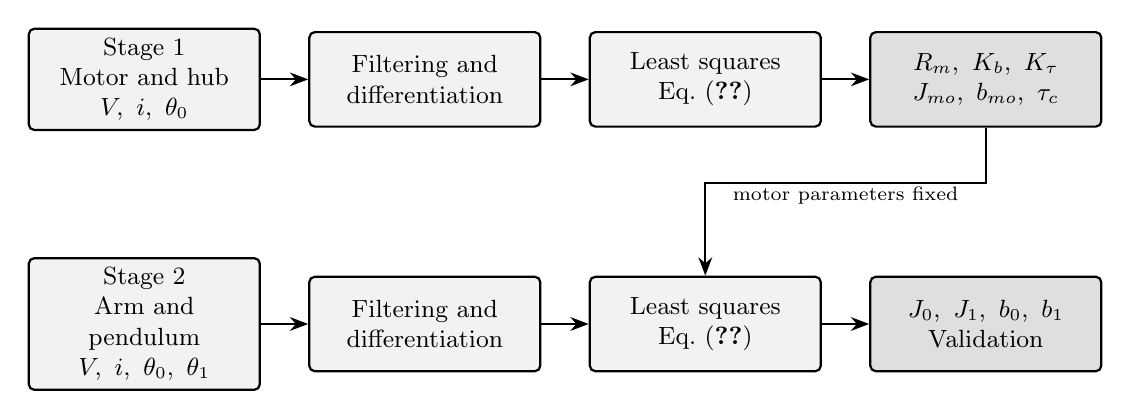
\begin{tikzpicture}[
  box/.style={draw, thick, rounded corners=2pt, fill=gray!10, align=center, font=\small, minimum height=1.2cm, text width=2.7cm},
  arr/.style={-{Stealth}, thick},
  node distance=0.6cm]
  \node[box] (s1) {Stage 1\\Motor and hub\\$V,\ i,\ \theta_0$};
  \node[box, right=of s1] (f1) {Filtering and\\differentiation};
  \node[box, right=of f1] (l1) {Least squares\\Eq.~\eqref{eq:motor_reg}};
  \node[box, right=of l1, fill=gray!25] (p1) {$R_m,\ K_b,\ K_\tau$\\$J_{mo},\ b_{mo},\ \tau_c$};
  \node[box, below=1.6cm of s1] (s2) {Stage 2\\Arm and pendulum\\$V,\ i,\ \theta_0,\ \theta_1$};
  \node[box, right=of s2] (f2) {Filtering and\\differentiation};
  \node[box, right=of f2] (l2) {Least squares\\Eq.~\eqref{eq:full_reg}};
  \node[box, right=of l2, fill=gray!25] (p2) {$J_0,\ J_1,\ b_0,\ b_1$\\Validation};
  \draw[arr] (s1) -- (f1); \draw[arr] (f1) -- (l1); \draw[arr] (l1) -- (p1);
  \draw[arr] (s2) -- (f2); \draw[arr] (f2) -- (l2); \draw[arr] (l2) -- (p2);
  \draw[arr] (p1.south) -- ++(0,-0.7) -| (l2.north);
  \node[font=\scriptsize, fill=white, inner sep=1pt] at ($(p1.south)!0.5!(l2.north) + (0,0.08)$) {motor parameters fixed};
\end{tikzpicture}
\caption{Two-stage parameter estimation procedure.}
\label{fig:stages}
\end{figure}

\end{document}
